\documentclass[border=3pt]{standalone}
\usepackage{amsmath}
\usepackage{tikz}
\usetikzlibrary{arrows.meta,positioning,fit,backgrounds,calc}
\begin{document}
    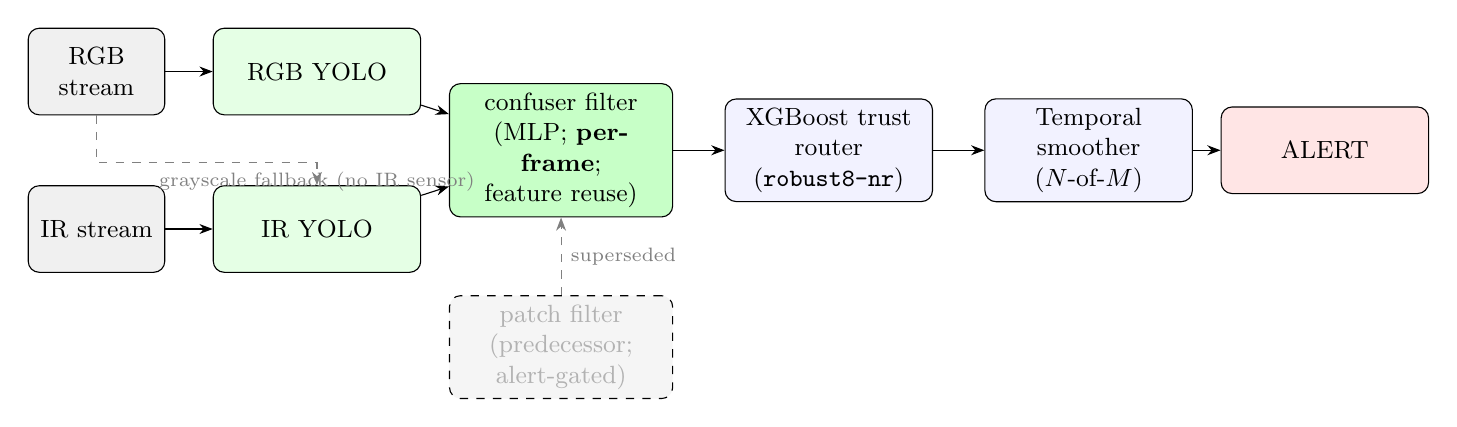
\begin{tikzpicture}[>=Stealth, font=\small,
      box/.style={draw, rounded corners, align=center, minimum height=11mm, text width=24mm, fill=blue!5},
      det/.style={box, fill=green!10},
      ver/.style={box, fill=green!22, text width=26mm},
      io/.style={box, fill=gray!12, text width=15mm},
      old/.style={draw, dashed, rounded corners, align=center, minimum height=10mm, text width=26mm, fill=gray!8, text=gray!60}]
      \node[io]  (rgb)  at (0,1.0)   {RGB stream};
      \node[io]  (ir)   at (0,-1.0)  {IR stream};
      \node[det] (ry)   at (2.8,1.0) {RGB YOLO};
      \node[det] (iy)   at (2.8,-1.0){IR YOLO};
      \node[ver] (ver)  at (5.9,0)   {confuser filter\\(MLP; \textbf{per-frame};\\feature reuse)};
      \node[box] (clf)  at (9.3,0)   {XGBoost trust\\router\\(\texttt{robust8-nr})};
      \node[box] (temp) at (12.6,0)  {Temporal\\smoother\\($N$-of-$M$)};
      \node[box, fill=red!10] (alert) at (15.6,0) {ALERT};
      \node[old] (patch) at (5.9,-2.5) {patch filter\\(predecessor; alert-gated)};
      \draw[->] (rgb)--(ry);   \draw[->] (ir)--(iy);
      \draw[->] (ry)--(ver);   \draw[->] (iy)--(ver);
      \draw[->] (ver)--(clf);  \draw[->] (clf)--(temp); \draw[->] (temp)--(alert);
      \draw[->, dashed, gray] (patch) -- node[right, font=\scriptsize, text=gray]{superseded} (ver);
      \draw[->, dashed, gray] (rgb.south) -- ($(rgb.south)+(0,-0.6)$) -| (iy.north)
            node[midway, below, font=\scriptsize, text=gray]{grayscale fallback (no IR sensor)};
    \end{tikzpicture}
\end{document}
